% LTeX: language=fr

\chapter{Rapport de stage}










\section{Introduction}

Mon stage s'est passé dans l'entreprise NRB, plus précisément dans l'équipe SecOps en charge de la sécurité opérationnelle dans l'entreprise et chez plusieurs clients. Grâce à ce stage en lié au processus forensique, c'est-à-dire à l'acquisition, l'analyse des données forensique et des menaces (malware, documents malicieux, etc.), j'ai pu grandement améliorer mes connaissances en informatique et en cybersécurité.

La mise en place d'une architecture pour l'infrastructure d'analyse des données forensiques a été une première pour moi, tout comme des aspects moins techniques comme la participation à des réunions ou la gestion de projet.





\section{Objectifs du stage}

L'objectif de ce stage était de créer une solution d'analyse contenant un ensemble d'outils pour améliorer les capacités de l'équipe SecOps en termes d'analyse forensique. Ça comprend aussi la détection et l'analyse de menaces, comme les emails, les documents ou les exécutables. Cette solution doit être isolée pour éviter la propagation des menaces. Il doit aussi pouvoir être facilement restauré dans un état initial. Un ensemble d’outils de forensique et d’analyse de menaces sont utilisés comme une sandbox, des outils d'analyse réseau, des logiciels de copie et montage disque, des scripts python, etc. Le tout dans un environnement virtualisé.

La mise en place de cet environnement doit bien entendu s'accompagner de la rédaction d'une documentation pour l'utilisation et la mise à jour de l'infrastructure et des outils qu'elle contient.





\section{Présentation de l'entreprise}



\subsection{NRB}

\textit{Network Research Belgium}, souvent abrégé sous la forme du sigle \textit{NRB} est une entreprise belge du secteur des TIC, les technologies de l'information et de la communication, fondée en 1987 en Belgique mais à vocation européenne. L'entreprise fournit des services dans les quatre domaines suivants:
\begin{itemize}
    \item la \textit{consultance} pour accompagner ses clients dans leurs démarches de transformation numérique et le conseil en cybersécurité;
    \item les \textit{services logiciels} comme le développement et la maintenance d'applications;
    \item les \textit{services infrastructures et clouds}, NRB permet à ses clients d'utiliser le cloud privé de NRB et les clouds publics d'IBM, Microsoft, Google et Amazon;
    \item les \textit{services de managed staffing} consistent à fournir du personnel à des entreprises qui en ont besoin pour conduire à bien leurs projets.
\end{itemize}

Certains de ces services sont fournis par les filiales du groupe NRB. En effet, NRB est un groupe qui s'agrandit notamment par des acquisitions d'entreprises dans le domaine technologique. En 2020, le groupe NRB comptait 3200 collaborateurs, avec un chiffre d'affaires de 413 millions d'euros.



\subsection{L'équipe SecOps}

SecOps vient de \textit{Sécurité et Opérations}, c'est l'équipe principale de gestion de la sécurité chez NRB. Comme l'indique le mot \textit{sécurité} de SecOps, ils doivent gérer les incidents de sécurité qui se produisent dans l'entreprise et chez certains de leurs clients mais ils ne gèrent pas l'ensemble des \textit{opérations}. Par exemple, lorsqu'une vulnérabilité a été détectée ce n'est pas leur rôle de mettre à jour le système d'exploitation ou de patcher l'application vulnérable, c'est le rôle de l'équipe qui est responsable de cette application ou système d'exploitation. Cependant, l'équipe SecOps a la responsabilité de trouver ces vulnérabilités et de vérifier qu'elles ont bien été corrigées.

L'équipe fonctionne en mode agile ce qui fait qu'il y a deux types de charges de travail. Premièrement, il y a le \textit{build}: c'est le fonctionnement normal où chacun avance sur ses projets et améliore les outils, les procédures, participe à des réunions et améliore la sécurité de NRB et de ses clients de manière générale. Deuxièmement, il y a le \textit{run} qui est assigné à une personne qui doit résoudre les tickets assignés à SecOps comme les incidents ou bien les demandes de changements dans l'infrastructure de l'entreprise qui doivent recevoir une autorisation de sécurité pour être implémentés. Par exemple, une demande pour donner les permissions administrateur sur une machine à un utilisateur est une demande de changement et un employé recevant un mail de phishing est un incident.

Le lundi, toutes les deux semaines, l'équipe SecOps se réunit pour ce qui est appelé le \textit{sprint review} de 15h30 à 17h30. Lors de cette réunion, chaque membre de l'équipe présente ce qu'il a accompli les deux semaines précédentes et ce qu'il a prévu de faire les deux semaines suivantes. Cependant, ce n'est pas la seule réunion effectuée à intervalle régulier parce qu'il y a aussi le \textit{daily standup}, réunion journalière de 8h30 à 9h, lors de laquelle on revoit les incidents de la veille avec un dashboard et ce que chacun a prévu de faire pour la journée.





\section{Journalier}

Pendant toute la durée du stage, j'ai envoyé un rapport d'avancement de stage à mon promoteur par mail pour l'informée de l'avancement du stage, des objectifs, des problèmes rencontrés et de ce que j'ai fait au jour le jour. Le tout était accompagné d'un petit résumé pour que ce soit plus facilement lisible. Dans cette section, je vais simplifier en mettant uniquement ce résumé pour chaque semaine plutôt que d'écrire le détail de ce qui a été fait chaque jour.



\subsection{Première semaine: 31 janvier - 25 février}

Pendant la première semaine, j'ai commencé à intégrer l'équipe, à participer aux réunions, découvrir les locaux, le fonctionnement de l'organisation, etc. J'ai défini les objectifs pour le stage ainsi qu'un premier planning, notamment avec un diagramme de Gantt. J'ai aussi effectué mes premières recherches sur les sandbox, j'ai surtout essayé de lister les sandbox existantes qu'elles soient gratuites ou commerciales.



\subsection{Deuxième semaine: 7 février - 11 février}

Pendant la deuxième semaine, j'ai passé une grande partie de mon temps à lire le cours SIFR (Security Incident First Responder) d'IBM qui avait été suivie par une partie des membres de l'équipe SecOps en avril 2021. Cette formation couvre les réflexes à avoir quand il y a un incident de sécurité comme l'acquisition de données forensiques et l'analyse de malware automatiquement avec une sandbox et manuellement avec des logiciels et des scripts.



\subsection{Troisième semaine: 14 février - 18 février}

Comme prévu, lors de cette troisième semaine, j'ai passé beaucoup de temps à faire des recherches sur le processus forensique ainsi que sur les outils utilisés lors de celui-ci. À la fin de la semaine, j'ai réussi à produire un rapport sur les outils dont la connaissance est à approfondir et les distributions qui les contiennent. J'ai aussi eu l'occasion de rencontrer un client de l'entreprise.



\subsection{Quatrième semaine: 21 février - 25 février}

Cette semaine, mon maître de stage fait le \textit{run}, il doit donc s'occuper des incidents de sécurité et valider les demandes de changements dans l'infrastructure NRB qui doivent recevoir une autorisation de sécurité. J'ai donc suivi ce qu'il faisait pour voir comment tout fonctionnait et il m'a donné quelques cas simples à résoudre pour me faire la main. J'ai aussi listé les besoins en infrastructure et les outils en fonction des use cases.



\subsection{Cinquième semaine: 28 février - 4 mars}

Lors de cette cinquième semaine, j'ai revu l'infrastructure d'analyse de données forensiques et de menaces. Il faut faire attention à bien isoler les machines d'analyse parce que les malwares pourraient potentiellement les infecter et à partir de là, se répandre dans le réseau de l'entreprise. J'ai aussi continué mes recherches sur les méthodes d'analyse forensiques, notamment en étudiant la méthode utilisée par Interpol.



\subsection{Sixième semaine: 7 mars - 11 mars}

Cette semaine, je me suis concentré sur le test des différents outils d'acquisition de données forensiques listés les semaines précédentes. J'ai aussi continué les recherches sur les méthodes d'analyse forensique en me concentrant sur les preuves d'exécution d'un programme dans un environnement Windows.



\subsection{Septième semaine: 14 mars - 18 mars}

L'architecture que j'ai proposée pour les machines d'analyse a été validée. Il faut évidemment faire attention parce que si une machine d'analyse de malware est compromise, elle pourrait infecter tout le réseau et il s'agit donc de bien les isoler pour réussir à protéger l'entreprise correctement. J'ai aussi commencé à avoir accès à NECS, le cloud de NRB pour y installer l'infrastructure. Enfin, j'ai continué à faire des recherches sur l'acquisition et l'analyse de données forensiques, en particulier comment empêcher un individu malintentionné d'altérer ou supprimer les traces de ses actions.



\subsection{Huitième semaine: 21 mars - 25 mars}

J'avais commencé à installer les machines d'analyse de données forensiques et de malwares dans le cloud en fin de semaine passée et j'ai continué à le faire cette semaine. Je n'ai pas pu terminer à cause de quelques problèmes techniques : problèmes de configuration DNS et la virtualisation imbriquée qui n'est pas activée sur l'infrastructure. J'ai aussi passé les deux derniers jours de la semaine pour assister dans l'acquisition et l'analyse forensique d'un PC avec d'autres membres de l'équipe SecOps.



\subsection{Neuvième semaine: 28 mars - 1 avril}

J'ai terminé l'analyse du PC Windows 11 que j'avais commencée la semaine passée et qui a un peu décalé mon planning mais m'a permis d'apprendre beaucoup de chose et surtout de mettre en pratique mon travail. Suite à cela, j'ai écrit la marche à suivre d'acquisition de données forensique puis j'ai continué à installer l'infrastructure de sandboxing sur NECS (le cloud NRB). Ce n'est pas tout à fait terminé à cause de quelques complications pour l'activation de la virtualisation imbriquée mais le gros du travail d'installation a été effectué.



\subsection{Dixième semaine: 4 avril - 8 avril}

J'ai pu commencer à tester la virtualisation imbriquée sur NECS (le cloud NRB), ce qui est nécessaire pour utiliser CAPEv2, le logiciel d'analyse de malware. Pour tester la sandbox, j'ai commencé à écrire un petit malware mais je ne l'ai pas encore terminé parce que je passe du temps à installer la sandbox, et ce n'est pas une tâche aisée.



\subsection{Onzième semaine: 11 avril - 15 avril}

Cette semaine, j'ai réussi à installer la sandbox correctement (il y avait des problèmes de configuration) et j'ai fait des tests pour vérifier son bon fonctionnement. J'attends le retour de l'équipe VMWare cher NRB pour déplacer la sandbox du tenant de test vers le tenant de production. Les retours sont bien sûr plus lents car ce sont les vacances de Pâques. J'ai aussi effectué l'analyse forensique d'un PC Windows 10 et d'une clé USB qui avaient été compromis par un malware. Ça a permis de tester les outils forensiques dans un cas réel et de trouver des problèmes. Par exemple, à cause du changement d'heure entre le moment où le PC a été infecté et le moment de l'analyse, certains timestamps étaient mal interprétés.



\subsection{Douzième semaine: 18 avril - 22 avril}

J'ai continué à travailler sur l'installation de la sandbox et les tests pour vérifier ses capacités une fois qu'elle sera installée. J'ai eu quelques problèmes avec la virtualisation imbriquée. La semaine passée, elle avait été activée sur une VM dans le tenant de développement pour effectuer des tests et voir si elle n'affecterait pas les autres machines virtuelles de l'environnement mutualisé. Cette semaine, on l'a activée sur une machine de l'environnement de production mais pas sur la bonne. J'ai donc commencé l'installation sur l'environnement de production avec du retard. J'ai aussi créé un test pour la sandbox, c'est un fichier Excel contenant une macro exécutant des commandes powershell, déposant un exécutable sur le système. C'est difficile à analyser manuellement mais facile avec une sandbox.



\subsection{Treizième semaine: 23 avril - 27 avril}

J'ai travaillé sur l'installation d'outils supplémentaires dans les VM d'analyse et la configuration de la sandbox pour qu'elle puisse analyser des fichiers Excel (et n'importe quel document Office d'ailleurs) mais je n'ai pas réussi. Après plusieurs jours sur l'affaire en fin de semaine, j'ai dû abandonner pour continuer à avancer dans mon travail. Le mardi, on a aussi testé le Digital Escape Game créé par l'équipe SecOps pour la mission diplomatique de l'AWEX en Grèce.



\subsection{Quatorzième semaine: 2 mai - 6 mai}

J'ai terminé de travailler sur les use cases d'analyse de malware et j'ai placé l'infrastructure sur le réseau isolé (pour pouvoir effectuer des analyses de malware). Ensuite, j'ai travaillé sur la documentation et j'ai terminé la partie analyse de malware, la partie analyse forensique est toujours en cours.



\subsection{Quinzième semaine: 9 mai - 13 mai}

Cette dernière semaine de stage, j'ai retravaillé la documentation que j'avais écrite pour utiliser l'infrastructure de sandboxing et pour la mettre à jour. J'ai aussi présenté les résultats de mon stage pour montrer ce que j'avais fait à l'équipe SecOps.





\section{Autres activités réalisées}



\subsection{Suivi du run, analyse d'un cas de phishing}

Lors de la semaine de \textit{run} de mon maître de stage, je l'ai un peu suivi pour voir comment se passe la résolution de tickets dans l'équipe SecOps. J'ai ainsi pu voir comment on fait pour vérifier si un changement au niveau du pare-feu doit être autorisé ou bien refusé. Autrement dit quand accepter un changement dans l'infrastructure.

Il m'a aussi donné des cas de phishing: la plupart des mails de phishing se font arrêter à l'entrée du réseau de NRB, cependant certains passent quand même de temps à autre. L'objectif de l'équipe SecOps est alors de trouver les utilisateurs impactés pour pouvoir les prévenir de ne pas ouvrir le mail et de ne pas cliquer sur les liens présents à l'intérieur. Il faut également vérifier que personne n'a ouvert ces liens. Grâce au proxy web, on peut voir qui a ouvert quels liens et ainsi mitiger les menaces.



\subsection{Analyse d'un malware}

Le vendredi 4 mars, avec un membre de l'équipe SecOps, nous avons analysé un malware qui avait été détecté et bloqué par Windows Defender alors qu'il se trouvait dans une archive zip. Nous avons lancé une analyse statique en utilisant l'outil PeStudio. Cela nous a permis de voir les informations comme la date de compilation qui aurait été réalisée en 2096... En observant le reste des propriétés statiques, force est de constater que le malware est obfusqué, c'est-à-dire qu'il cache une partie de son code et le chargera lui-même au moment de l'exécution pour empêcher ou tout du moins compliquer l'analyse statique.

Après avoir copié son hash sur \textit{virustotal} et des sandboxes gratuites en ligne comme \textit{any.run}, nous avons pu observer que ce malware avait déjà été soumis sur ces sites en 2019. Grâce à l'analyse dynamique fournie par ces services, nous savons qu'il lance un autre processus en utilisant \textit{rundll32.exe}, c'est une technique populaire des auteurs de malwares pour donner l'impression que leur processus est légitime, car bien que la librairie exécutée est la leur, le processus est lancé avec un exécutable Windows. Ce cheval de Troie va également chercher les adresses IP de deux domaines et les contacter. Tous ces indicateurs de compromissions sont utiles pour vérifier qu'aucune machine dans le parc informatique n'a été infectée.



\subsection{Analyse forensique d'un PC Windows}

Fin mars, l'équipe SecOps de NRB a eu un cas où elle devait analyser un PC Windows 11 pour essayer de comprendre un incident. J'ai eu la chance de pouvoir y participer et tester les outils que j'avais sélectionnés. Après avoir fait une capture RAM avec \textit{Belkasoft RAM Capturer}, j'ai enchaîné avec une image disque à l'aide de \textit{FTK Imager}.

Une fois l'acquisition des données forensiques effectuée, il a fallu lancer quelques programmes utilisés pour la réponse à incident comme \textit{Process Explorer} et \textit{Autoruns} de la suite d'outils de \textit{Sysinternals} (voir figures \ref{fig:autoruns} et \ref{fig:process-explorer}). En analysant un par un les processus en train de tourner et les traces de persistance sur l'ordinateur, on peut espérer retrouver un malware qui tourne ou aurait tourné sur la machine.

Finalement, j'ai analysé les données forensiques avec \textit{Autopsy} et \textit{Volatility 3}. Comme les disques étaient chiffrés avec BitLocker (une technologie Microsoft de chiffrement de disque dur), il a fallu monter l'image disque en lecture seule sur le PC d'analyse avec \textit{Arsenal Image Mounter}. On peut ensuite déchiffrer les disques avec les clés BitLocker récupérées préalablement sur l'ordinateur et analyser le disque déchiffré dans Autopsy.

\begin{figure}
    \centering
    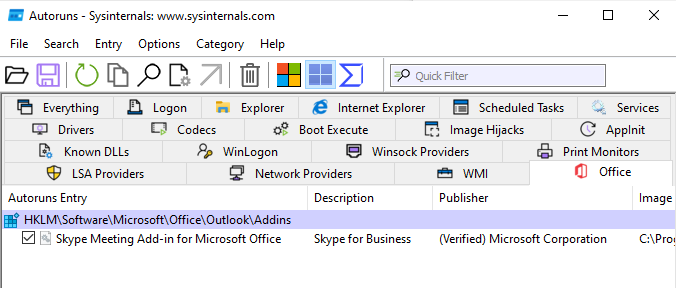
\includegraphics[width=0.75\linewidth]{images/incident-response/IR-autoruns.png}
    \caption{Logiciel \textit{Autoruns} de la suite \textit{Sysinternals} utilisé dans le cadre d'une réponse à incident.}
    \label{fig:autoruns}
\end{figure}

\begin{figure}
    \centering
    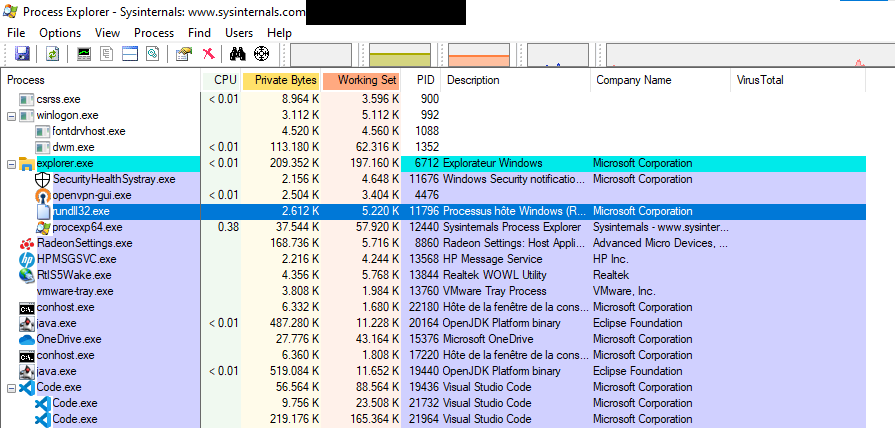
\includegraphics[width=0.99\linewidth]{images/incident-response/IR-process-explorer.png}
    \caption{Logiciel \textit{Process Explorer} de la suite \textit{Sysinternals} utilisé dans le cadre d'une réponse à incident.}
    \label{fig:process-explorer}
\end{figure}



\subsection{Analyse d'une clé USB infectée}

Mi-avril, j'ai eu l'occasion d'analyser une clé USB infectée. Le fonctionnement du malware est intéressant parce qu'il est simple et efficace. Quand on branche la clé sur le PC, l'explorateur de fichiers s'ouvre sur la racine du système de fichiers qui ne contient qu'un "Lecteur USB" comme vous pouvez le voir sur la figure \ref{fig:infected-usb-key}. En fait, il s'agit d'un raccourci qui exécute un script caché. Ce script lance l'installation d'un malware et ouvre une nouvelle fenêtre explorer dans le dossier caché \textit{Lecteur USB} pour tromper l'utilisateur.

Bien que les options pour afficher les extensions de noms de fichiers et les éléments masqués soient sélectionnées, on ne voit ni l'extension du raccourci, ni les éléments masqués. C'est parce qu'en plus d'avoir l'attribut \textit{Hidden}, les éléments cachés ont l'attribut \textit{System} qui n'est normalement possédé que par des fichiers et dossiers nécessaires au bon fonctionnement de Windows. Le paramètre pour les afficher malgré tout se trouve dans le \textit{Control Panel}.

\begin{figure}
    \centering
    \makebox[\textwidth]{
        \resizebox{17cm}{!}{
            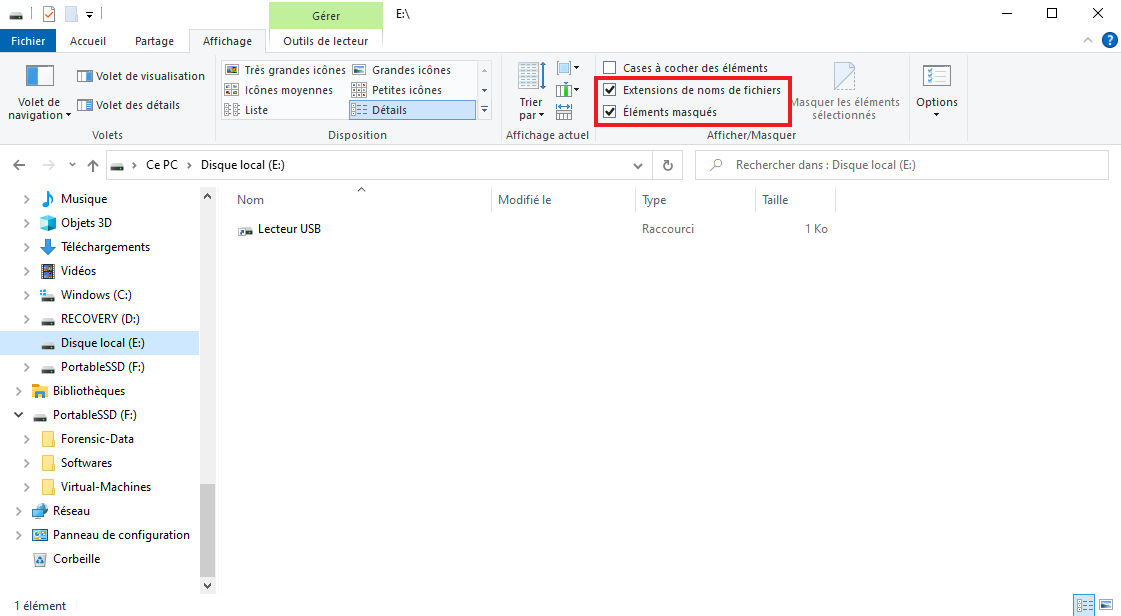
\includegraphics[width=0.99\linewidth]{images/infected-usb-key/explorer-listing.png}
        }
    }
    \caption{Racine de la clé USB infectée dans l'explorateur de fichiers.}
    \label{fig:infected-usb-key}
\end{figure}

Après avoir effectué une image disque de la clé USB, j'ai lancé une analyse avec le logiciel Autopsy qui a scanné l'ensemble de l'image et retrouvé des éléments supprimés. En fait, parce que le système de fichier est du FAT32, quand on déplace un dossier, il est supprimé et recréé à cet autre endroit. On peut le voir sur la figure \ref{fig:autopsy-moved-folders}, où le dossier \textit{Documents} a été déplacé de la racine du système de fichier vers l'intérieur du dossier \textit{Lecteur USB}. Dans ce cas-ci, c'est très intéressant parce que ça nous informe que:
\begin{itemize}
    \item La clé USB était utilisée normalement auparavant.
    \item Elle a été infectée par un PC qui appartient sans doute à la victime.
    \item Donc l'infection du PC est potentiellement antérieure à l'infection de la clé.
\end{itemize}

\begin{figure}
    \centering
    \makebox[\textwidth]{
        \resizebox{10cm}{!}{
            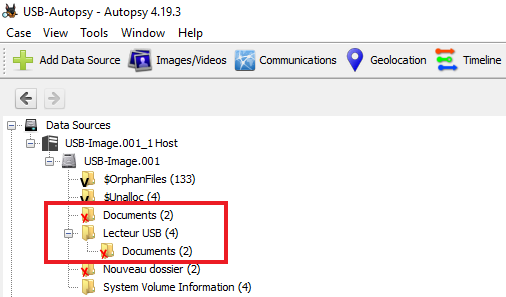
\includegraphics[width=0.99\linewidth]{images/infected-usb-key/autopsy-moved-folders.png}
        }
    }
    \caption{Analyse d'un déplacement de dossier sur la clé USB.}
    \label{fig:autopsy-moved-folders}
\end{figure}





\section{Résultats}

J'ai décidé de diviser cette section en deux parties: l'analyse de malware et l'analyse forensique. Bien que l'analyse de malware fasse partie de l'analyse forensique et que les solutions aux deux problèmes soient liées, il y a eu un grand effort pour travailler ce sujet lors du TFE et je pense donc que c'est plus intéressant de séparer les résultats ici.



\subsection{Analyse de malware}

L'analyse de malware peut être réalisée de manière automatique avec la plateforme d'analyse automatique FAME qui a été mise en place, ainsi que la sandbox. On peut y mettre des emails, des documents, des exécutables et encore d'autres types de fichiers. Il y a cependant des problèmes avec l'analyse automatique dynamique des documents Office avec la sandbox parce que la machine virtuelle imbriquée, infectée volontairement pour monitorer le document, plante complètement. Malgré ces soucis, on peut tout de même tout analyser, y compris les documents Office, avec la plateforme d'analyse automatique FAME. Les analyses effectuées sur ces documents ne pourront cependant être que statiques et pas dynamiques.

En plus de la sélection des outils et de leur mise en place, une infrastructure a été pensée pour isoler les machines virtuelles d'analyse et de la documentation a été écrite pour pouvoir mettre à jour les outils et les utiliser. Ces outils et ces marches à suivre ont été testés sur plusieurs use cases et avec des cas concrets par moi-même et plusieurs membres de l'équipe SecOps.



\subsection{Acquisition et analyse forensique}

Cette section s'appelle \textit{acquisition et analyse forensique} parce que j'ai sélectionné et installer des logiciels d'acquisition des données forensiques comme la mémoire volatile et la mémoire de masse et parce que j'ai aussi effectué des recherches sur les outils et les procédures d'analyse de ces données. Pour que les procédures puissent être suivies par d'autres membres de l'équipe SecOps à l'avenir, j'ai écrit de la documentation sur l'utilisation de tous ces outils et les informations intéressantes qui peuvent en être extraites.

J'ai eu la chance lors de ce stage d'avoir pu participer à deux enquêtes forensiques sur des systèmes Windows et une clé USB avec d'autres membres de l'équipe SecOps, ce qui a été très enrichissant tant d'un point de vue social que technique. Par ces occasions, j'ai pu confronter les outils et les procédures d'acquisition et d'analyse forensique à la réalité et ne pas rester uniquement dans la théorie.





\section{Améliorations possibles}



\subsection{Analyse de malware}

L'apport de ce stage concernant l'analyse de malwares est principalement concentré sur la mise en place d'outils d'analyse automatique dans une infrastructure isolée. Et parce que l'infrastructure est isolée, c'est plus difficile de déplacer des fichiers à analyser du PC de l'analyste vers la machine virtuelle d'analyse. Ainsi, on pourrait pousser l'automatisation encore plus loin en soumettant automatiquement des éléments potentiellement malveillants ce qui ferait gagner du temps aux analystes. Après discussion avec des membres de l'équipe SecOps, ça pourrait être fait avec la plateforme d'automatisation Splunk SOAR.

Toujours concernant l'analyse de malwares, ou plutôt l'analyse de maldocs, c'est-à-dire des documents malicieux, la machine virtuelle utilisée par le logiciel CAPE Sandbox plante lorsqu'on essaie de les lancer. Ce serait une bonne amélioration de corriger cela pour pouvoir effectuer une analyse dynamique sur ces documents. La création d'une machine virtuelle Linux pour analyser des malwares qui ne fonctionnent que sur les systèmes Linux est aussi une piste d'amélioration intéressante.

Enfin, l'analyse manuelle de logiciels malveillants pourrait aussi être approfondie. C'est une tâche qui ne sera sans doute pas effectuée tous les jours étant donné que ça pourrait faire perdre beaucoup de temps inutilement. Mais malgré tout, il faudra dans certains cas entrer plus en profondeur dans l'analyse du malware. Par exemple dans le cas où un PC a été compromis et on veut comprendre ce qu'il a fait sur le système et comment le détecter sur d'autres machines au sein de l'environnement. Travailler plus cet aspect-là peut donc être intéressant.



\subsection{Analyse forensique}

Pour ce qui est de l'analyse forensique, en plus d'approfondir l'analyse forensique des systèmes Windows, il est aussi possible d'étendre l'éventail des systèmes qu'on peut analyser comme en s'attaquant aux systèmes Linux et macOS.

Les machines d'analyse se trouvent dans un environnement virtualisé, ce qui est très pratique et flexible. Cependant, il crée également des contraintes. Par exemple, le temps de transfert des données forensiques vers l'infrastructure d'analyse peut être lent, ce qui peut faire perdre un temps crucial lors d'analyses, particulièrement en-dehors de l'entreprise. C'est pour ça qu'avoir un PC portable pour effectuer des analyses forensiques peut être intéressant. Il faut aussi utiliser des SSD portables, rapides et de grande capacité pour pouvoir stocker les données forensiques et les résultats d'analyse. De plus, pour analyser les clés USB, une solution de Write-Blocker physique, dans lequel on peut brancher une clé USB et ainsi empêcher l'écriture accidentelle sur la clé est un outil supplémentaire à envisager.





\section{Diagrammes de Gantt}

Comme vous pouvez le voir, au début, j'avais des difficultés à réaliser mon premier diagramme de Gantt. D'abord, c'était la première fois que je me prêtais à cet exercice mais je manquais aussi d'informations pour que le diagramme de Gantt soit précis. J'ai donc laissé certaines tâches globales pendant plusieurs semaines plutôt que de les rediviser en plus petites tâches. En présentant ce planning à mon maître de stage, mais aussi à l'équipe SecOps en entier lors d'une réunion de sprint review, j'ai pu avoir des retours. Ça m'a aidé à mieux cerner le but du stage et modifier ce que j'avais prévu de faire pour m'aligner sur ces objectifs.

Lorsque j'ai à nouveau créé un diagramme de Gantt, en milieu de stage, une partie du stage avait déjà été réalisée et la roadmap était beaucoup plus claire dans mon esprit. Grâce à ce nouveau diagramme, j'ai pu à nouveau communiquer. Cette fois, c'était surtout avec mon maître de stage pour valider les priorités et s'assurer que les objectifs du stage puissent être atteints.

Enfin, le dernier diagramme de Gantt permet surtout de faire le point sur ce qui a été fait, identifier avec du recul les tâches qui ont pris le plus de temps et revoir les points bloquants qui ont ralenti la progression du travail.

\begin{figure}
    \centering
    \noindent
    \makebox[\textwidth]{
        \resizebox{19cm}{!}{
            \includestandalone{images/gantt-chart/gantt-chart}
        }
    }
    \caption{Diagrammes de Gantt réalisés à différentes périodes du stage.}
    \label{fig:gantt-diagrams}
\end{figure}





\section{On Stage}

\begin{figure}
    \centering
    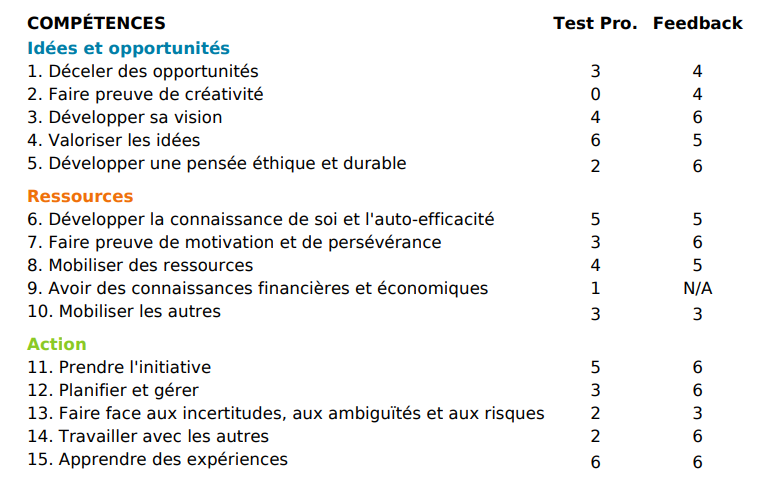
\includegraphics[width=0.85\linewidth]{images/onstage/onstage-skills.png}
    \caption{Résultats de la plateforme On Stage.}
    \label{fig:onstage}
\end{figure}

Comme vous pouvez le voir sur la figure \ref{fig:onstage}, parmis mes points faibles, il y a se confronter aux incertitudes, les connaissances financières et économiques, ainsi que mobiliser les autres. Mes points forts se trouvent plutôt dans la section \textit{Action}, par exemple: apprendre de mes expériences, travailler avec les autres, la planification.





\section{Critique du stage}

Grâce à ce stage, j'ai maintenant une meilleure compréhension du monde professionnel et du fonctionnement des grandes entreprises mais aussi de l'importance de la cybersécurité dans ce milieu et comment la mettre en place. J'ai aussi pu acquérir de nombreuses compétences en informatique et plus spécifiquement en termes de forensique, d'analyse de malware et en architecture de solutions.

La solution que j'ai apportée à l'entreprise pourra être utilisée pour analyser les tentatives de pénétration avec des mails de phishing ou des exécutables de manière automatique, ce qui fera gagner du temps aux analystes et leur permettra de rentrer plus en profondeur pour mieux prévenir les menaces. Au niveau de l'analyse forensique des systèmes contaminés, j'ai pu répondre aux attentes en termes de procédures et de la sélection d'outils, que j'ai d'ailleurs pu tester dans des situations réelles.

J'ai rencontré un point négatif, comme c'est souvent le cas dans une grande entreprise, on est dépendant d'autres équipes. Ça a ralenti la progression du travail, notamment quand on doit faire travailler plusieurs équipes ensemble et qu'il faut trouver un moment de libre pour amener tout le monde ensemble dans une réunion.

En revanche, l'avantage de faire de la cybersécurité dans une grande entreprise est qu'on peut avoir l'opportunité de communiquer avec beaucoup de personnes et de toucher à beaucoup de technologies. Un autre avantage, c'est que l'équipe SecOps est elle est plutôt jeune et dynamique. Elle est en pleine croissance et il y a toujours beaucoup de choses à faire et à entreprendre.





\section{Conclusion}

Ce stage m'a beaucoup apporté et a été une expérience professionnelle très enrichissante. Il m'a permis d'en apprendre beaucoup plus d'un point de vue technique bien entendu, surtout dans le domaine de la forensique, de l'analyse de malware ou plus généralement dans le fonctionnent de Windows. Mais j'ai aussi retenu des leçons sur l'organisation: lister les objectifs à atteindre, créer une liste de tâches pour les atteindre et estimer le temps que chacune va prendre. Ensuite, en communiquant avec d'autres personnes, on peut avoir un retour et corriger le planning. C'est d'ailleurs quelque chose qu'il faut faire régulièrement pour résoudre les problèmes qui vont invariablement arriver et réorienter le travail pour atteindre les objectifs.

D'ailleurs, en faisant ce stage, j'ai mieux compris à quel point la communication était importante. En particulier, parce que NRB est une grande entreprise, elle est divisée en plusieurs plus petites équipes et j'ai dû interagir avec certaines d'entre elles pour pouvoir accomplir mes tâches. J'ai aussi eu l'occasion de travailler avec des clients. Et bien sûr, j'ai beaucoup communiqué avec le reste de l'équipe. D'abord lors des réunions qui étaient organisées tous les jours mais aussi en dehors.


